% Page de titre pour les annexes
\chapter*{Annexes}
\addcontentsline{toc}{chapter}{Annexes}
\thispagestyle{plain}
\clearpage

% Diagramme de modules fonctionnels - Paysage
\begin{landscape}
\thispagestyle{empty}
\begin{figure}[p]
\centering
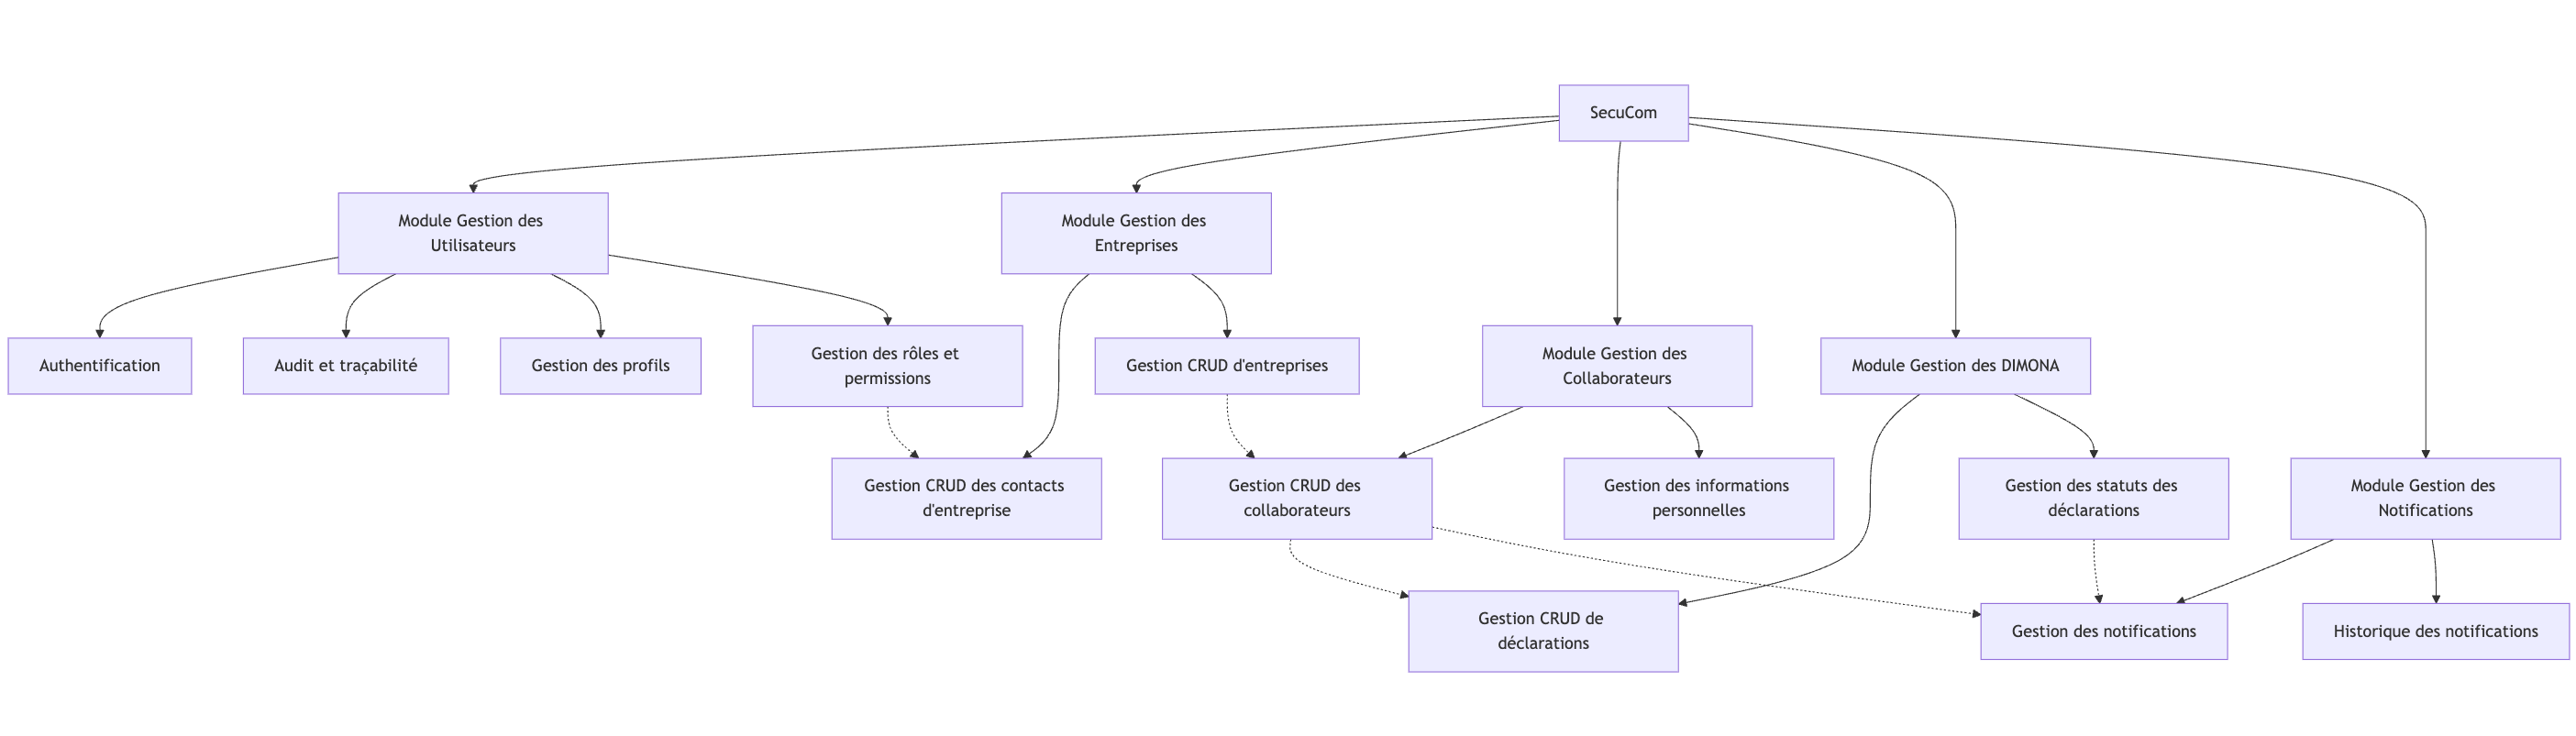
\includegraphics[width=0.85\paperheight,height=0.8\paperwidth,keepaspectratio]{ComposantsDiagram.png}
\caption{Diagramme de modules fonctionnels de SecuCom}
\end{figure}
\end{landscape}

% Diagramme de classes - Paysage
\begin{landscape}
\thispagestyle{empty}
\begin{figure}[p]
\vspace*{-1cm}
\centering
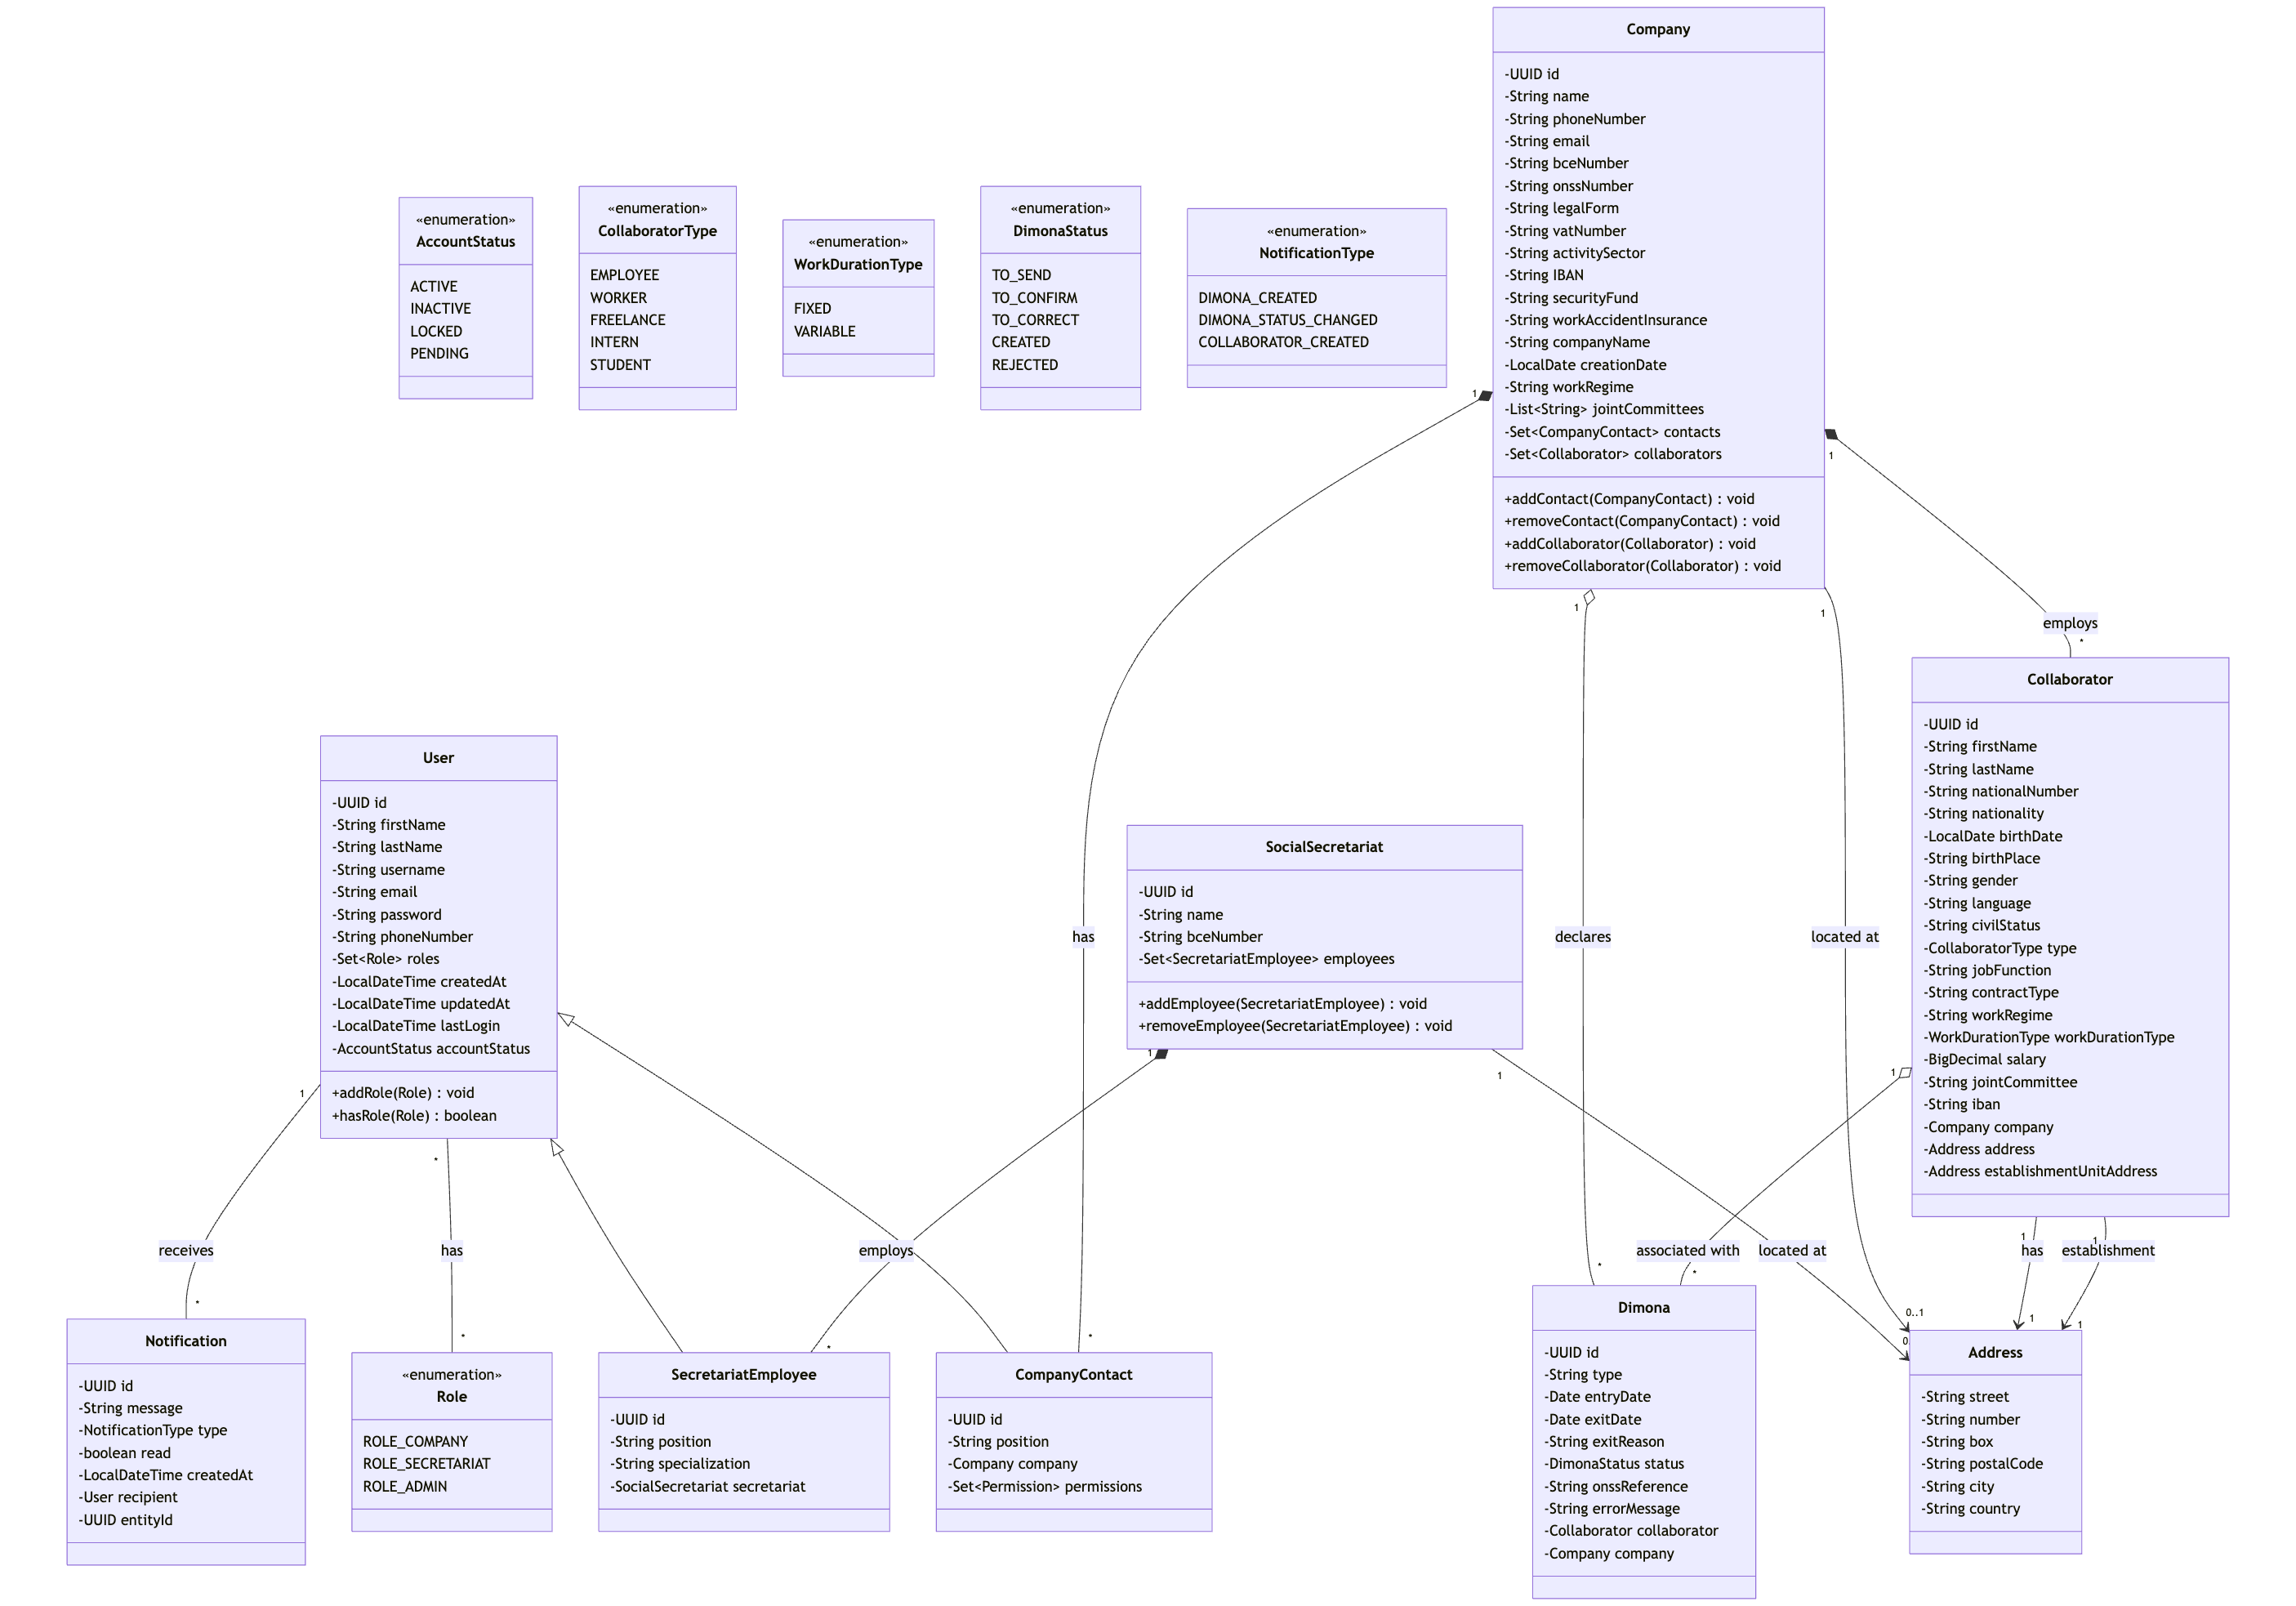
\includegraphics[width=0.9\paperheight,height=0.85\paperwidth,keepaspectratio]{ClassDiagram.png}
\caption{Diagramme de classes de SecuCom}
\vspace*{1cm}
\end{figure}
\end{landscape}

% Diagramme d'entités relationnelles - Portrait
\thispagestyle{empty}
\vspace*{-2cm}
\begin{center}
\makebox[\textwidth][c]{
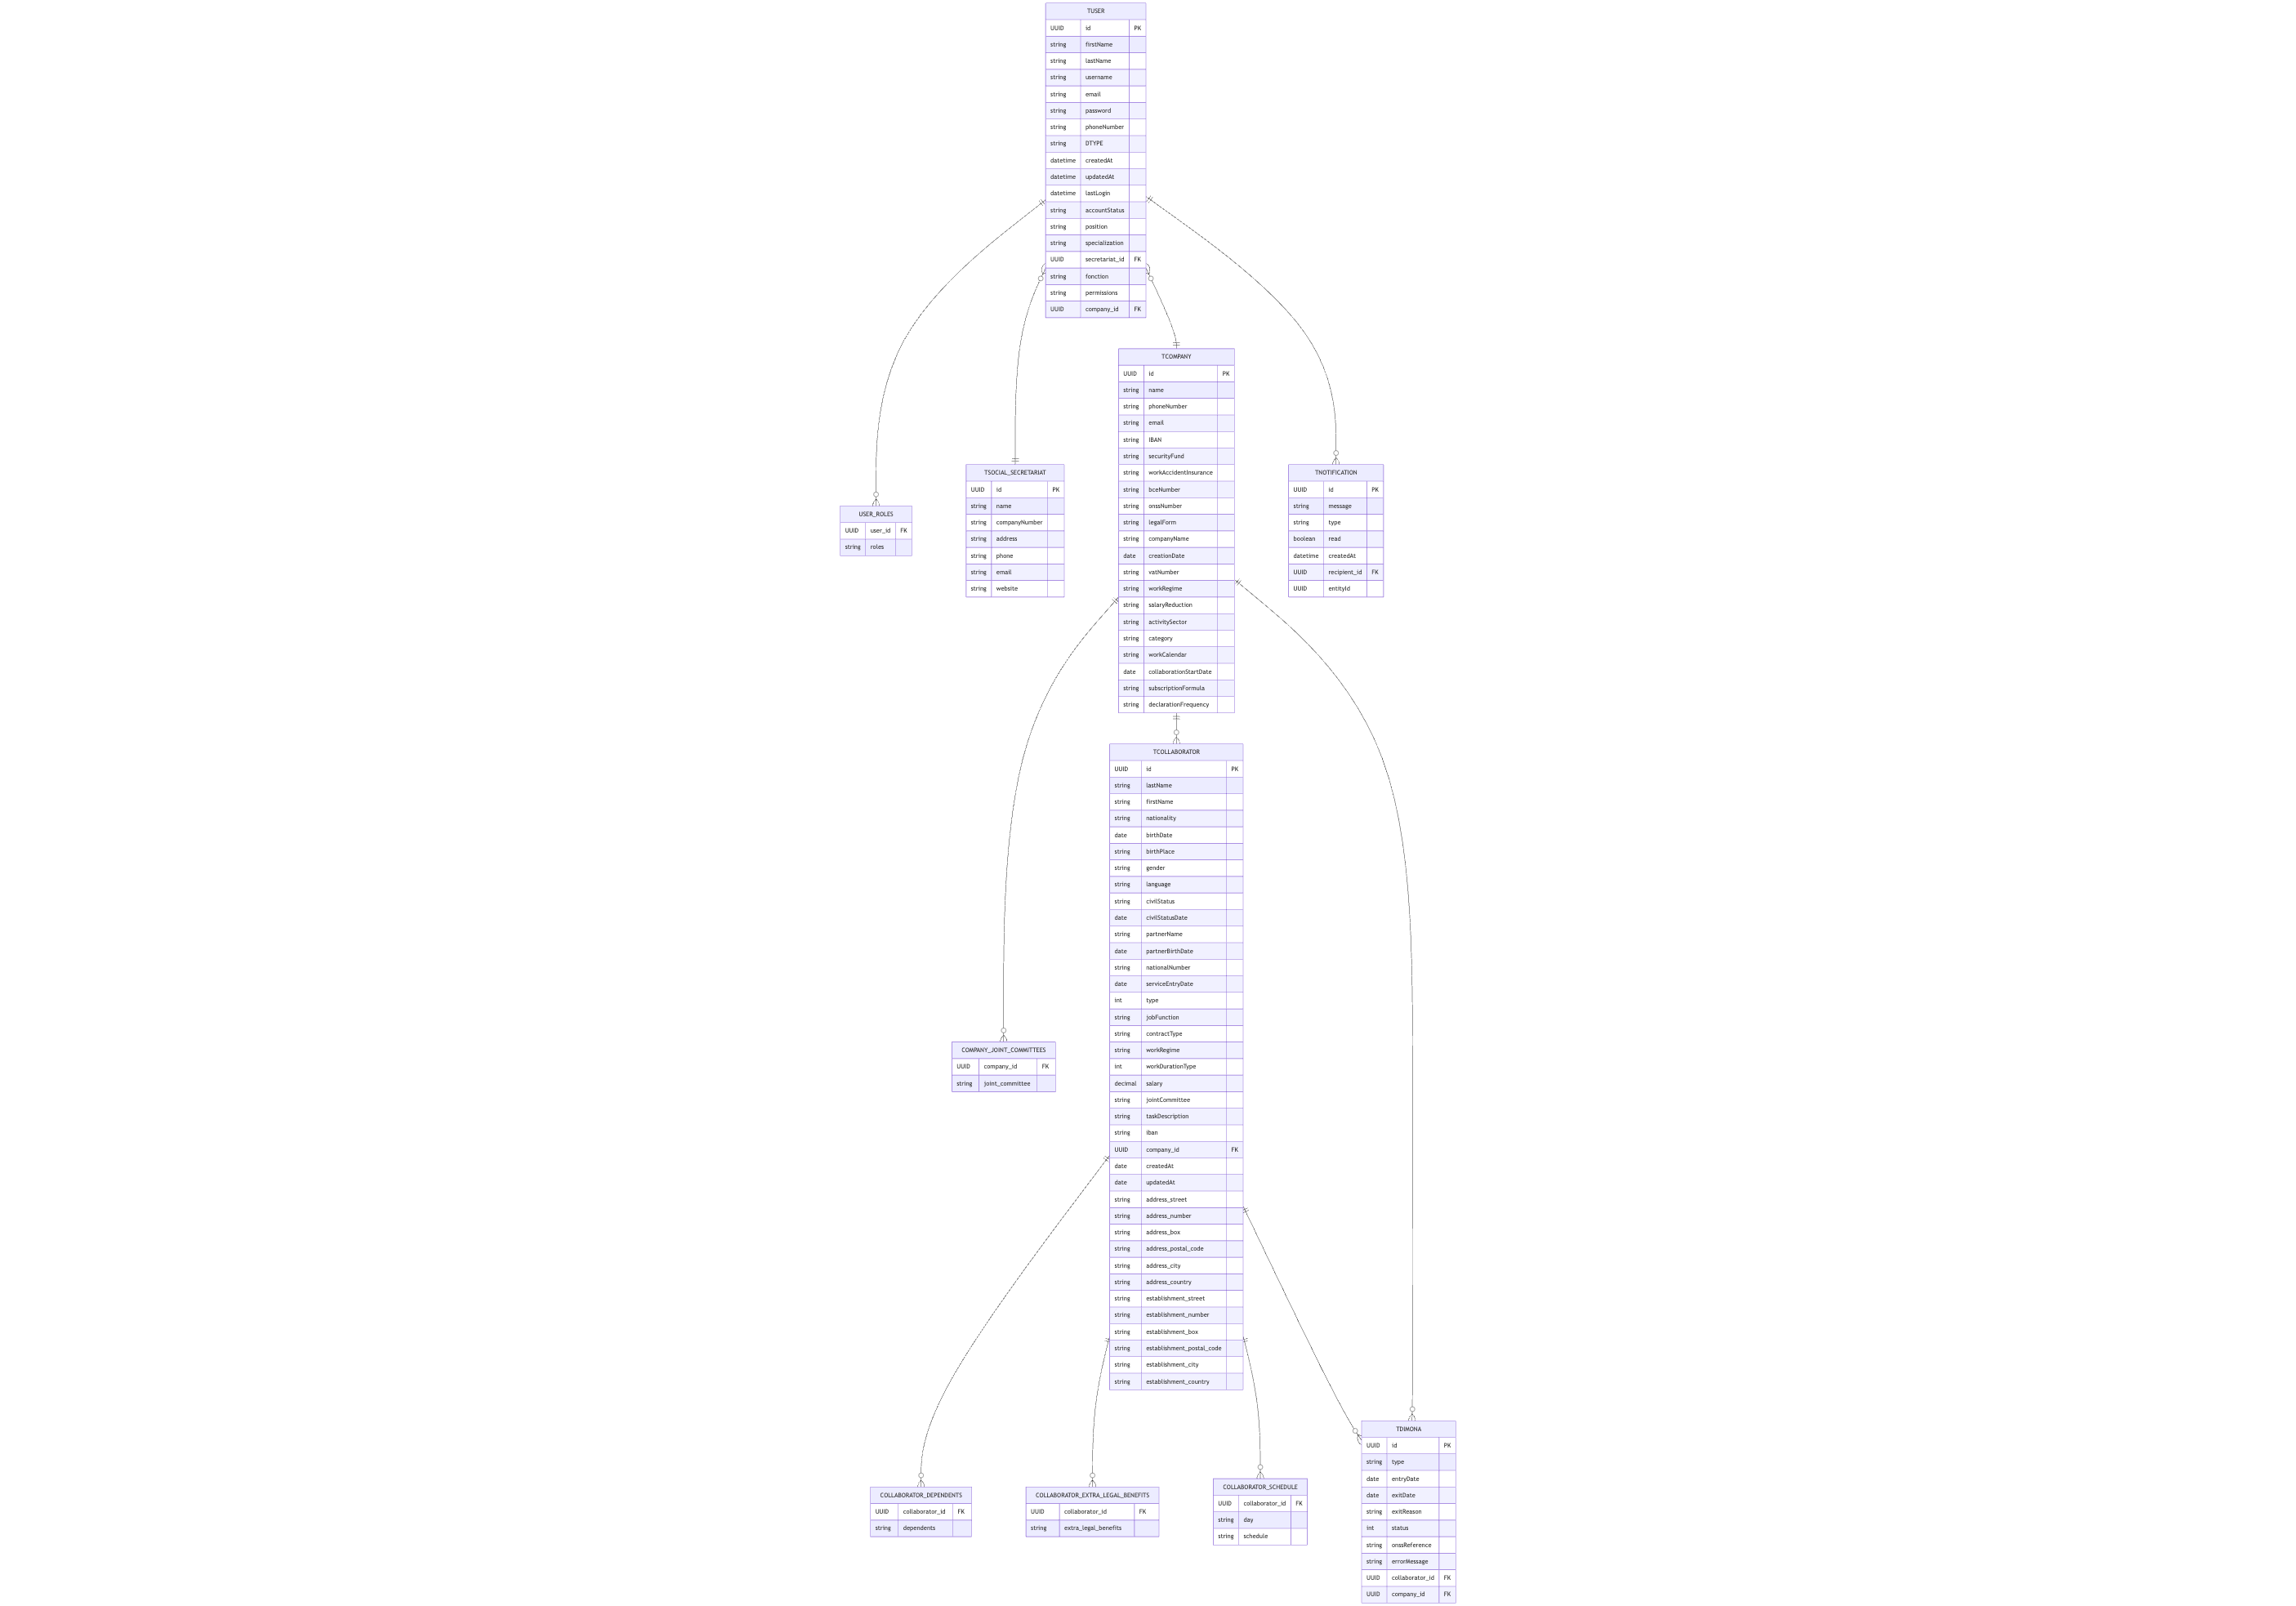
\includegraphics[width=2\textwidth,height=0.8\textheight]{ERD.png}
}
\vspace{1cm}
\captionof{figure}{Diagramme d'entités relationnelles}
\end{center}
\clearpage

% Diagramme de séquence - Portrait
\thispagestyle{empty}
\vspace*{-2cm}
\begin{center}
\makebox[\textwidth][c]{
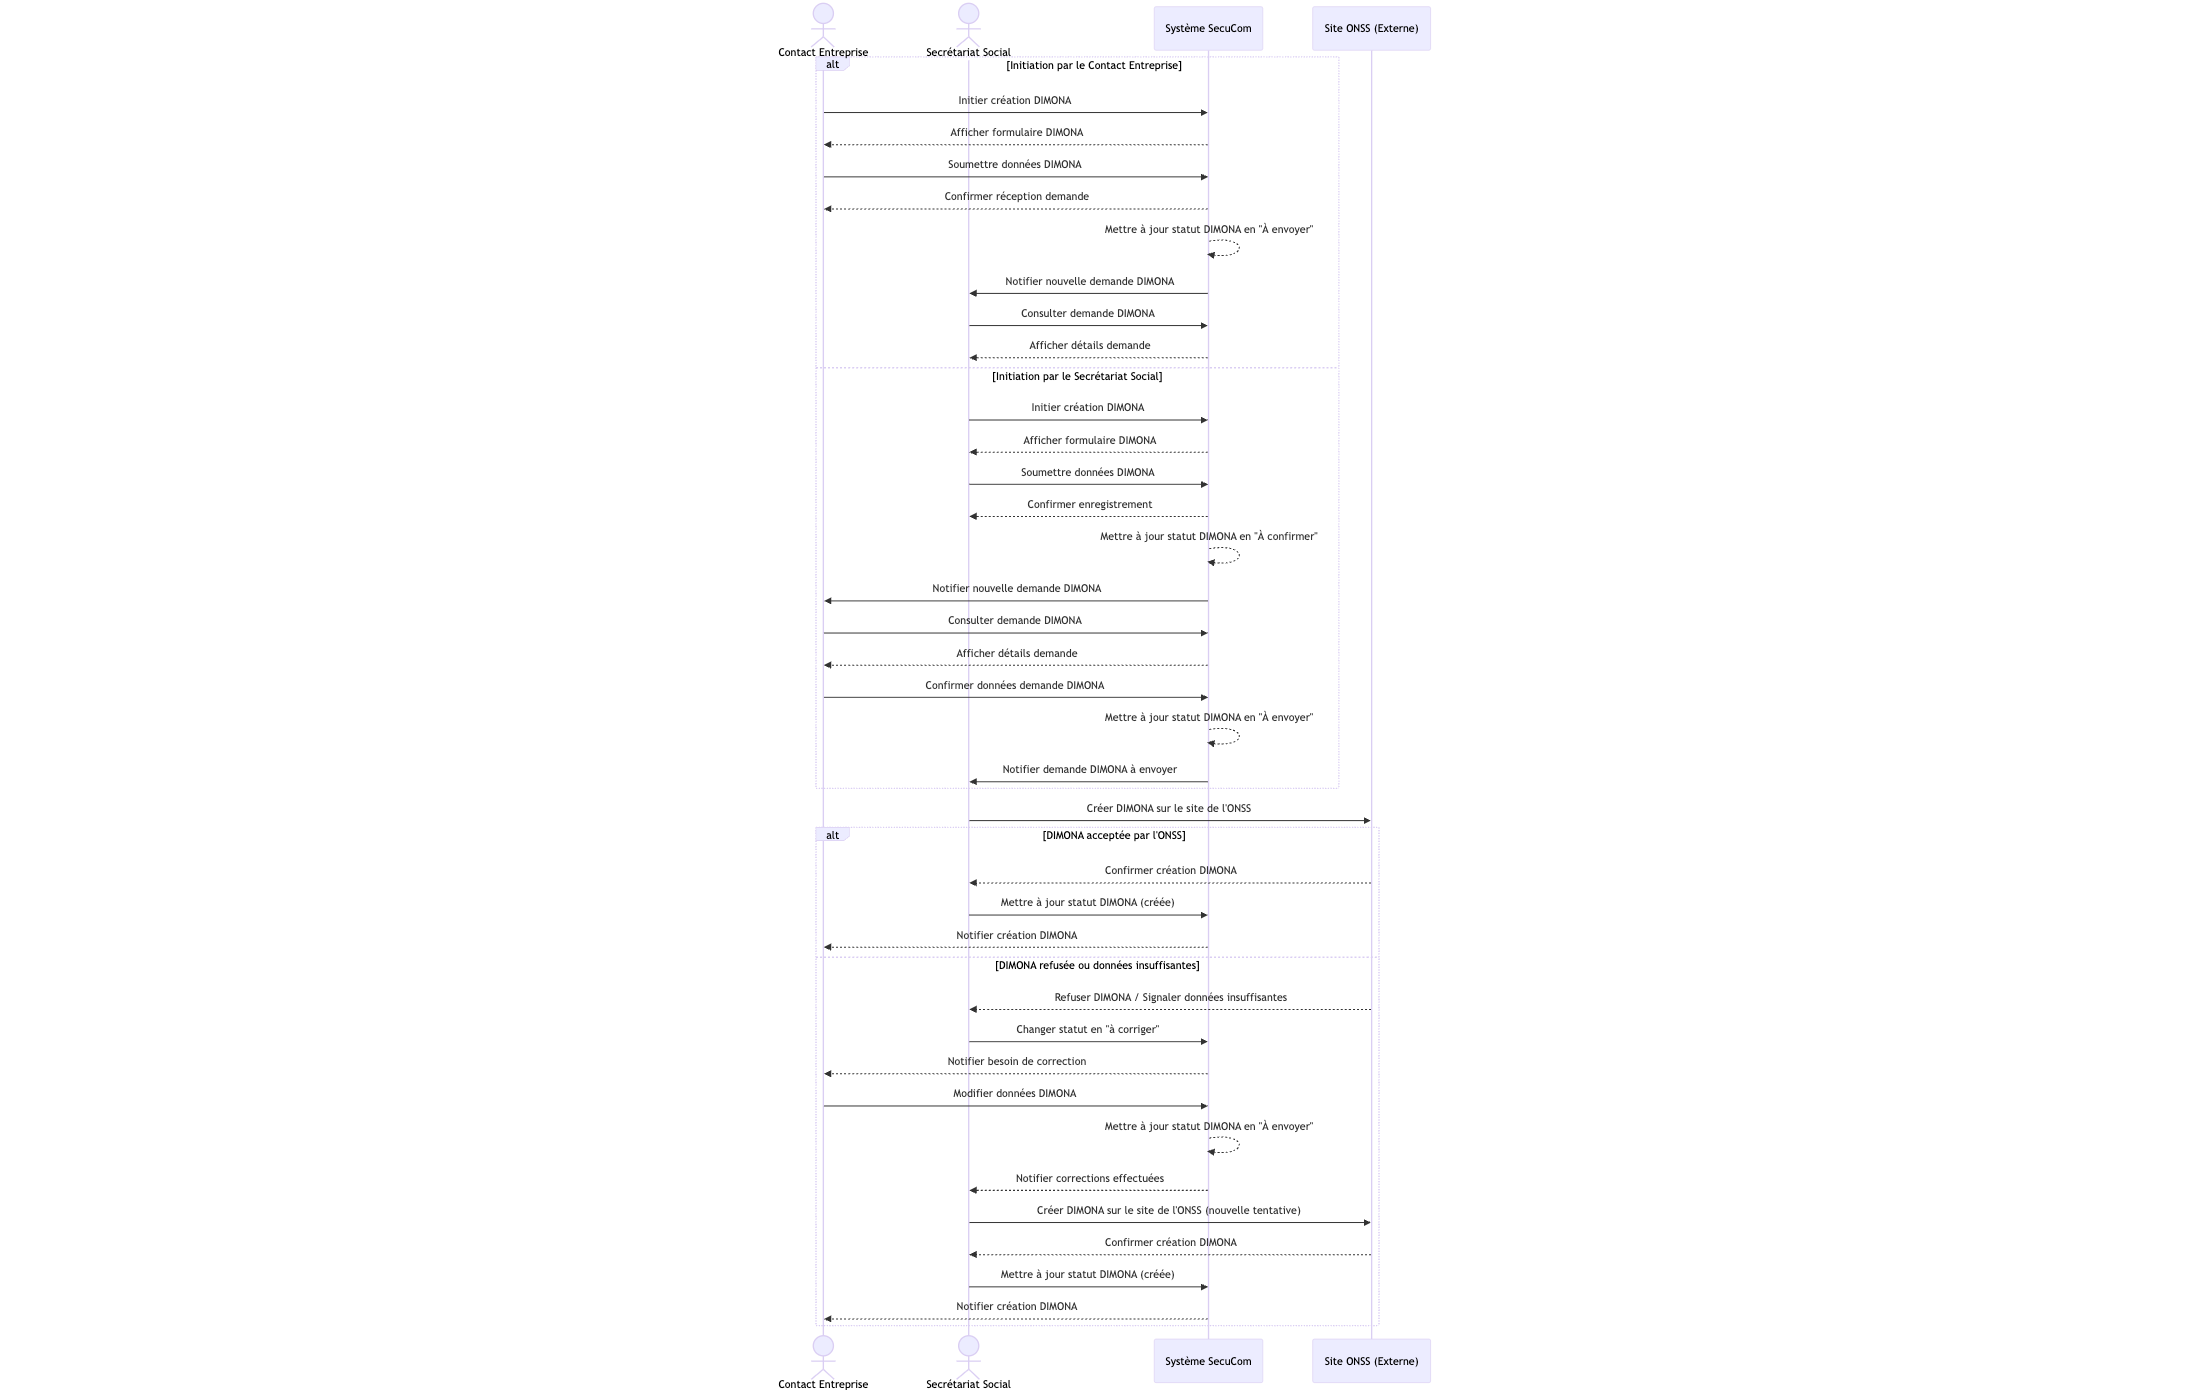
\includegraphics[width=2\textwidth,height=0.8\textheight]{SD_creation_dimona.png}
}
\vspace{1cm}
\captionof{figure}{Diagramme de séquence - Création d'une déclaration DIMONA}
\end{center}
